% !TEX program = xelatex
\documentclass[10pt,letterpaper,twocolumn]{article}

% === GEOMETRY ===
\usepackage[top=0.75in, bottom=0.75in, left=0.75in, right=0.75in]{geometry}

% === FONTS ===
\usepackage{fontspec}
\usepackage{unicode-math}
\setmainfont{Latin Modern Roman}[
  Extension=.otf,
  UprightFont=lmroman10-regular,
  BoldFont=lmroman10-bold,
  ItalicFont=lmroman10-italic,
  BoldItalicFont=lmroman10-bolditalic,
]
\setsansfont{Latin Modern Sans}[
  Extension=.otf,
  UprightFont=lmsans10-regular,
  BoldFont=lmsans10-bold,
  ItalicFont=lmsans10-oblique,
  BoldItalicFont=lmsans10-boldoblique,
]
\setmonofont{Latin Modern Mono}[
  Extension=.otf,
  UprightFont=lmmono10-regular,
  ItalicFont=lmmono10-italic,
  Scale=0.85,
]
\newfontfamily\acbold{ywft-processing-bold}[
  Path=../../system/public/type/webfonts/,
  Extension=.ttf
]

% === PACKAGES ===
\usepackage{xcolor}
\usepackage{titlesec}
\usepackage{enumitem}
\usepackage{booktabs}
\usepackage{tabularx}
\usepackage{fancyhdr}
\usepackage{hyperref}
\usepackage{xurl}
\usepackage{graphicx}
\usepackage{ragged2e}
\usepackage{microtype}
\usepackage{natbib}
\usepackage{tikz}
\usetikzlibrary{arrows.meta, positioning}
\usepackage[colorspec=0.92]{draftwatermark}

% === COLORS ===
\definecolor{acpink}{RGB}{180,72,135}
\definecolor{acpurple}{RGB}{120,80,180}
\definecolor{acdark}{RGB}{64,56,74}
\definecolor{acgray}{RGB}{119,119,119}
\definecolor{acgreen}{RGB}{70,200,90}
\definecolor{draftcolor}{RGB}{180,72,135}

% === DRAFT WATERMARK ===
\DraftwatermarkOptions{
  text=WORKING DRAFT,
  fontsize=3cm,
  color=draftcolor!18,
  angle=45,
  pos={0.5\paperwidth, 0.5\paperheight}
}

% === HYPERREF ===
\hypersetup{
  colorlinks=true,
  linkcolor=acpurple,
  urlcolor=acpurple,
  citecolor=acpurple,
  pdfauthor={@jeffrey},
  pdftitle={Taking Turf: Aesthetic Computer on a Slopped Internet, the Prompt Corpus, and a Game Boy Garden},
}

% === SECTION FORMATTING ===
\titleformat{\section}
  {\normalfont\bfseries\normalsize\uppercase}
  {\thesection.}
  {0.5em}
  {}
\titlespacing{\section}{0pt}{1.2em}{0.3em}

\titleformat{\subsection}
  {\normalfont\bfseries\small}
  {\thesubsection}
  {0.5em}
  {}
\titlespacing{\subsection}{0pt}{0.8em}{0.2em}

% === HEADER/FOOTER ===
\pagestyle{fancy}
\fancyhf{}
\renewcommand{\headrulewidth}{0pt}
\fancyhead[C]{\footnotesize\color{draftcolor}\textit{Working Draft --- not for citation}}
\fancyfoot[C]{\footnotesize\thepage}

% === LIST SETTINGS ===
\setlist[itemize]{nosep, leftmargin=1.2em, itemsep=0.1em}
\setlist[enumerate]{nosep, leftmargin=1.2em}

% === COLUMN SEPARATION ===
\setlength{\columnsep}{1.8em}

% === PARAGRAPH SETTINGS ===
\setlength{\parindent}{1em}
\setlength{\parskip}{0.3em}

\tolerance=800
\emergencystretch=1em
\hyphenpenalty=50

\newcommand{\ac}{\textsc{Aesthetic.Computer}}

\begin{document}

\twocolumn[{%
\begin{center}
{\acbold\fontsize{26pt}{30pt}\selectfont\color{acdark} taking {\color{acgreen}turf}{\color{acpink}.}}\par
\vspace{0.5em}
{\normalfont\small\itshape\color{acpink} Aesthetic Computer on a Slopped Internet --- the Prompt Corpus, the Agent-Legible Canvas, and a Game Boy Garden}\par
\vspace{0.6em}
{\normalsize\href{https://prompt.ac/@jeffrey}{@jeffrey}}\par
{\small\color{acgray} Aesthetic.Computer}\par
{\small\color{acgray} ORCID: \href{https://orcid.org/0009-0007-4460-4913}{0009-0007-4460-4913}}\par
\vspace{0.3em}
{\small\color{acpurple} \url{https://aesthetic.computer/prompt} \enspace$\cdot$\enspace 2026-09-03}\par
\vspace{0.6em}
\rule{\textwidth}{1.5pt}
\vspace{0.5em}
\end{center}

\begin{center}
{\small\color{draftcolor}\textbf{[ working draft --- not for citation ]}}
\end{center}
\vspace{0.3em}

\begin{quote}
\small\noindent\textbf{Abstract.}
This paper answers a strategy question posed inside \ac{}~\citep{scudder2026ac} on September 3, 2026: \emph{given the current status quo of the internet, what is the best thing Aesthetic Computer can do to take more turf --- and earn its keep?} The status quo is measurable and strange. Most new web content is machine-generated~\citep{sailop2026state,abhs2026dead}, organic reach through search and feeds has collapsed~\citep{digitalbloom2026crisis,omnibound2026seo}, and the traffic that is growing is not human at all: AI agents now dominate request volume on many sites~\citep{datadome2026q2,workos2026majority}, while a counter-market in certified human work grows in parallel~\citep{npr2026cert}. We ground the argument in first-party evidence --- \ac{}'s own hit table, 4.78 million recorded piece loads whose top twenty rows contain both beloved instruments and vulnerability scanners probing for VPN logins --- and note what the platform deliberately does \emph{not} record: the raw text people type at the prompt. From this we argue for two moves that are one strategy. First, an \emph{agent-legible canvas}: a public MCP surface where any AI chat session can publish a KidLisp piece~\citep{scudder2026kidlisp} and hand its human a live URL, priced in credits at the moment of creation. Second, a \emph{Game Boy garden}: a side site where games for the original Game Boy are grown in public --- seeded small, mutated tick by tick by agents and players, playable in the browser at every stage --- and harvested as physical cartridges any user can order, flashed in-house or through the homebrew scene's production services~\citep{insidegadgets2026shop,nintendodiff2026gb}. The browser end claims the new machine-readable layer of the web; the cartridge end sells the one thing slop cannot be: a finished object that leaves the feed.
\end{quote}
\vspace{0.5em}
}]

\section{Introduction}

Turf, on the old internet, meant a position in a feed or a rank in a search index. Both of those markets are being repriced to nothing. The feeds are saturated with machine-generated filler that audiences have learned to name and resent~\citep{meltwater2026slop,forbes2026fans}, and the search index increasingly answers questions itself instead of sending the click~\citep{omnibound2026seo}. Meanwhile a genuinely new kind of visitor has arrived in volume: software agents that browse, call tools, and hand URLs back to the people they work for~\citep{humansec2026agentic,datadome2026q2}.

\ac{} is a small, live, URL-addressable creative computer~\citep{scudder2026ac,scudder2026urltradition}. It is not going to out-post the slop, and it should not try. The question this paper takes seriously is where the \emph{defensible} ground is for a platform whose unit of content is a running program rather than a static artifact --- and how holding that ground can pay for itself~\citep{scudder2026sustainability}.

The answer proposed here has two ends, deliberately far apart. At the fast end, \ac{} should become the easiest canvas for the agentic web to paint on: a public, metered MCP surface that turns any AI conversation into an authoring session ending in a live piece. At the slow end, it should grow games for a 1989 handheld in a public garden and sell the harvest as physical cartridges. These sound like opposite gestures. They are the same gesture at two speeds: both make the work \emph{live and claimable} in a way machine-generated static content structurally is not.

\section{The Slopped Internet, Measured}

Four measurements define the 2026 status quo (Table~\ref{tab:statusquo}).

\begin{table}[t]
\centering
\small
\begin{tabularx}{\columnwidth}{>{\raggedright\arraybackslash}X r}
\toprule
\textbf{Measurement} & \textbf{Value} \\
\midrule
Estimated share of new web content that is AI-generated~\citep{abhs2026dead,sailop2026state} & 52--90\% \\
``AI slop'' mentions, 2025 vs.\ 2024~\citep{meltwater2026slop} & $9\times$ \\
Organic click-share change, Jan 2025--Jan 2026~\citep{digitalbloom2026crisis} & $-11$ to $-23$\,pp \\
CTR drop when an AI Overview appears~\citep{omnibound2026seo} & $-61\%$ \\
AI-agent requests, Q2 2026, one bot-defense network~\citep{datadome2026q2} & 17.7\,B \\
Agent share of traffic, top B2B research pages~\citep{workos2026majority} & $\leq$42\% \\
Sites declaring machine-readable AI preferences~\citep{discoveredlabs2026webmcp} & $\sim$4\% \\
Sites exposing MCP server cards~\citep{discoveredlabs2026webmcp} & $<15$ \\
Authors Guild ``Human Authored'' titles, year one~\citep{npr2026cert} & 5{,}000+ \\
\bottomrule
\end{tabularx}
\caption{The status quo, September 2026. The first block is the slop flood and the collapse of organic reach; the second is the agentic traffic layer arriving before the web is ready for it; the last row is the counter-market in verified human work.}
\label{tab:statusquo}
\end{table}

First, the flood: estimates of the machine-generated share of new content range from roughly half to nine-tenths depending on methodology~\citep{abhs2026dead,sailop2026state}, and the audience has noticed --- ``slop'' went from niche complaint to word-of-the-year material, with negative sentiment majorities in social listening~\citep{meltwater2026slop,fortune2026slopwar}.

Second, the collapse of the old distribution: when an AI answer engine handles a query, most of the click volume that used to reach websites simply does not arrive~\citep{omnibound2026seo,digitalbloom2026crisis}. Positioning in feeds and indexes is land whose price is falling toward its true value.

Third, the new visitor: agentic traffic grew 45\% in a single quarter on one measurement network~\citep{datadome2026q2}, agents are already the dominant traffic source on many research-heavy pages~\citep{workos2026majority}, and the protocol layer has settled --- MCP for tools, with WebMCP entering a Chrome origin trial~\citep{devto2026standards,discoveredlabs2026webmcp}. Yet almost no sites are legible to these visitors: about 4\% declare AI preferences and fewer than fifteen expose MCP server cards~\citep{discoveredlabs2026webmcp}. That is a land rush where nearly all the land is unclaimed.

Fourth, the counter-market: as the flood rises, \emph{verified human} work becomes a premium good. The Authors Guild certified over five thousand titles as human-authored in its first year~\citep{npr2026cert}; badge systems and verification services multiply~\citep{notbyai2026,edtech2026verify}; broadcast research finds 90\% of listeners --- including AI users --- want their media made by people~\citep{nurdd2026humans}.

The strategic reading: \textbf{the new turf is (a) being a tool agents call, and (b) making artifacts whose humanity and liveness are verifiable.} Everything proposed below is one of those two claims staked.

\section{First-Party Evidence: What People Enter}

Strategy grounded only in industry reports would be borrowed conviction. \ac{} has its own instruments. Since December 31, 2025, the production server has recorded an anonymous hit for every piece load it serves, bucketed daily (\texttt{piece-hits}, written by \texttt{index.mjs} on each resolved request). As of September 3, 2026 the top 100 pieces account for 4{,}782{,}776 recorded loads. Table~\ref{tab:hits} shows the head of the distribution.

\begin{table}[t]
\centering
\small
\begin{tabularx}{\columnwidth}{@{}l r >{\raggedright\arraybackslash}X@{}}
\toprule
\textbf{Piece} & \textbf{Hits} & \textbf{Reading} \\
\midrule
\texttt{prompt} & 4{,}617{,}114 & the front door; 96.5\% of all recorded load \\
\texttt{+CSCOE+/logon.html} & 20{,}429 & scanners probing for Cisco SSL-VPN \\
\texttt{laer-klokken} & 18{,}923 & community clock piece \\
\texttt{notepat} & 10{,}331 & instrument~\citep{scudder2026notepat} \\
\texttt{+webvpn+/index.html} & 9{,}802 & more VPN scanner probes \\
\texttt{nopaint} & 8{,}935 & painting system \\
\texttt{\$bop} & 3{,}711 & KidLisp code (highest of 63 in top 100) \\
\texttt{starfield} & 2{,}020 & classic piece \\
\texttt{api/.env} & 1{,}791 & scanners fishing for leaked secrets \\
\texttt{prutti} & 1{,}682 & piece \\
\bottomrule
\end{tabularx}
\caption{Selected rows from the top of the \ac{} hit table, 2025-12-31 through 2026-09-03. Human instruments, KidLisp \$codes, and automated vulnerability scanners share the same leaderboard: the slopped internet is visible in our own logs. Full 100-row export: \texttt{data/piece-hits-2026-09-03.csv}.}
\label{tab:hits}
\end{table}

Three findings.

\textbf{The prompt is the product.} Across 163 recorded days the prompt averaged 28{,}326 loads per day, peaking at 74{,}343 on August 29, 2026. Whatever \ac{} does next, it happens at a command line that already has an audience.

\textbf{The dead internet visits us too.} Rows two, five, and nine of Table~\ref{tab:hits} are not people. They are automated scanners requesting Cisco VPN login paths and \texttt{.env} secrets files, absorbed by the catch-all router and dutifully recorded as ``pieces.'' Machine traffic probing for weaknesses outranks all but a handful of our most-loved human pieces. This is the status quo of Section 2 observed from our own porch, and it usefully calibrates the rest of the argument: much of the web's traffic is machines already --- the only question is whether the machines that visit you are burglars or patrons.

\textbf{The long tail is KidLisp.} Sixty-three of the top 100 pieces are stored KidLisp \texttt{\$codes} --- 72{,}961 combined loads of tiny, sourced, forkable programs. The platform has 17{,}538 stored codes and 2{,}969 registered handles. The \texttt{\$code} is already the platform's native, viral unit.

\subsection{What we do not store --- and should, carefully}

A natural question: does \ac{} store everything people \emph{type} at the prompt, including the attempts that resolve to nothing? It does not. Hits are recorded server-side per resolved load; raw prompt keystrokes, failed commands, and misspelled wishes are never persisted, and the platform's analytics policy (\texttt{shared/posthog-policy.mjs}) explicitly excludes ``source, prompts, media, filenames, handles, or artifact contents'' from third-party capture. The privacy stance is real. But it means the prompt is a search engine that discards its query log --- we cannot currently see what people \emph{wanted} that does not exist yet, which is the single most valuable product-direction signal a command-line system can have.

The proposal is a deliberate, privacy-first middle path: log \emph{unresolved} prompt tokens as anonymous daily aggregate counts only --- no session binding, no user binding, no ordering, no free-text retention beyond the token itself --- alongside the resolved-hit counts we already keep. The corpus of misses becomes a public instrument (``most-wished-for pieces this month'') rather than surveillance.

\section{Move One: The Agent-Legible Canvas}

The first claim to stake is the machine-readable layer, while it costs nothing. \ac{} is unusually shaped for it: a KidLisp piece is small enough for a language model to emit whole in a single completion, and the platform already turns stored source into a live URL and a short \texttt{\$code}~\citep{scudder2026kidlisp}. No build step, no scaffold, no asset pipeline. Among creative platforms this property is nearly unique --- and the plumbing exists: the repository already carries an MCP endpoint (\texttt{mcp-remote.mjs}) and a public storage API (\texttt{store-kidlisp.mjs}).

Concretely: publish an MCP server card and \texttt{llms.txt} on \texttt{aesthetic.computer}; expose \texttt{publish\_kidlisp}, \texttt{get\_source}, and \texttt{preview} as public MCP tools; enroll the prompt in the WebMCP origin trial~\citep{discoveredlabs2026webmcp}. Every AI chat session in the world becomes a potential \ac{} authoring session that ends with a human receiving a living, forkable URL instead of another static image.

The keep-earning half is priced at creation, not consumption. Agentic visitors browse enormously but buy almost nothing at checkout~\citep{humansec2026agentic}, so charging agents as shoppers is a dead end; charging their \emph{operators} for making and keeping things is not. Anonymous rate-limited \texttt{\$codes} stay free --- that is the funnel, and 17{,}538 stored codes prove it works. API keys with credit packs price the durable goods: named \texttt{@handle/piece} slots, persistence guarantees, HD renders and tapes, airtime on the TV stream.

\section{Move Two: The Game Boy Garden}

The second claim is staked at the opposite speed, on the counter-market: verifiable, live, finishable, \emph{physical} work~\citep{npr2026cert,nurdd2026humans}.

\textbf{The proposal.} A side site --- working name \emph{gameboygarden} --- where games for the original Game Boy are \emph{grown} rather than released. Each game is a plot. A seed is the smallest playable thing: one screen, one mechanic, a few kilobytes of compiled C~\citep{gbdk2020}. Growth happens in ticks: a small mutation --- a new room, a new enemy, a tune --- proposed by an agent or a human contributor, committed, compiled to a ROM by CI, and immediately playable in the browser through a WebAssembly emulator. Visitors water plots (votes that steer the next mutation) and take cuttings (forks). Every tick is a commit, a playable diff, and a short reel for the feeds. The garden metaphor is not decoration; it is a publishing cadence and an honest account of latency. KidLisp pieces are one-completion-sized; Game Boy games are grown-over-months-sized. The two moves bracket the platform's range.

\begin{figure*}[t]
\centering
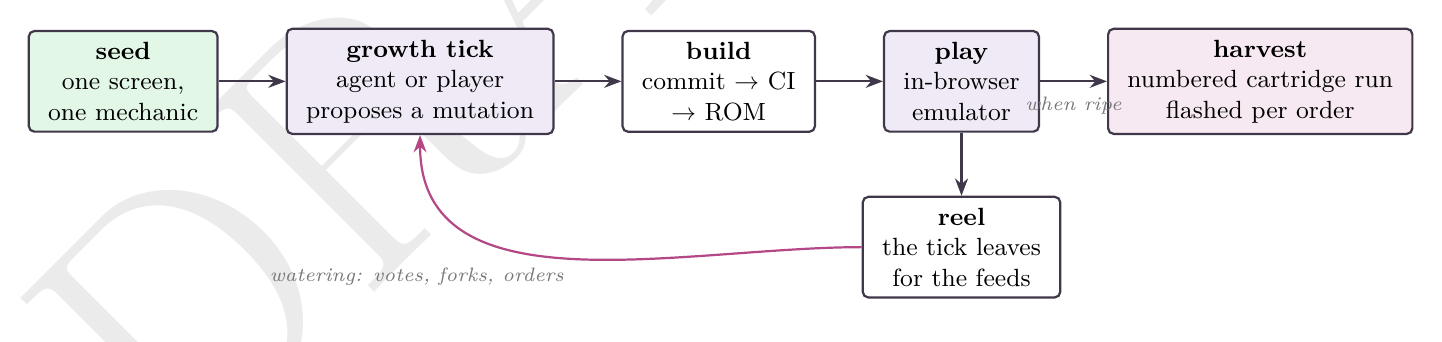
\begin{tikzpicture}[
  node distance=0.55cm and 0.85cm,
  every node/.style={font=\small},
  plot/.style={draw=acdark, thick, rounded corners=2pt, align=center,
    minimum height=2.4em, inner xsep=0.7em, inner ysep=0.4em},
  flow/.style={-{Stealth[length=2.2mm]}, thick, acdark},
  loop/.style={-{Stealth[length=2.2mm]}, thick, acpink},
  lab/.style={font=\scriptsize\itshape, text=acgray}
]
\node[plot, fill=acgreen!15] (seed) {\textbf{seed}\\one screen,\\one mechanic};
\node[plot, right=of seed, fill=acpurple!12] (tick) {\textbf{growth tick}\\agent or player\\proposes a mutation};
\node[plot, right=of tick] (build) {\textbf{build}\\commit $\rightarrow$ CI\\$\rightarrow$ ROM};
\node[plot, right=of build, fill=acpurple!12] (play) {\textbf{play}\\in-browser\\emulator};
\node[plot, right=of play, fill=acpink!12] (harvest) {\textbf{harvest}\\numbered cartridge run\\flashed per order};
\node[plot, below=0.8cm of play] (reel) {\textbf{reel}\\the tick leaves\\for the feeds};
\draw[flow] (seed) -- (tick);
\draw[flow] (tick) -- (build);
\draw[flow] (build) -- (play);
\draw[flow] (play) -- node[lab, below=2pt] {when ripe} (harvest);
\draw[flow] (play) -- (reel);
\draw[loop] (reel.west) to[out=180, in=270] node[lab, below left] {watering: votes, forks, orders} (tick.south);
\end{tikzpicture}
\caption{The garden loop. Every growth tick is simultaneously a commit, a playable build, and a piece of outbound media carrying a door back to the plot; the feeds are top-of-funnel for a URL, never the destination. Harvest --- a physical cartridge --- is the one state slop cannot reach.}
\label{fig:loop}
\end{figure*}

\textbf{Why the Game Boy.} The homebrew scene is real, growing, and underserved by exactly this format: at least 51 physical Game Boy releases shipped in 2025, up from 5 in 2018, at 45--70\,EUR per cartridge~\citep{nintendodiff2026gb}; new titles crowdfund routinely~\citep{gamerant2026stains,timeextension2025physical}; and a modern compatible handheld, the ModRetro Chromatic, is in current manufacture~\citep{modretro2026}. The toolchain is mature and scriptable~\citep{gbdk2020,gbstudio2026}, ROMs are 32\,KB--1\,MB, and the aesthetic performs absurdly well in short vertical video --- a distribution machine \ac{} already operates daily. Nobody in the scene has ``watch games grow in public'' as a site.

\textbf{The cartridge harvest.} When a plot ripens, any user can order it as a physical cartridge (Table~\ref{tab:carts}): flashed in-house on writable carts with a USB flasher~\citep{insidegadgets2026shop,adafruit2026flashing}, custom-labeled at small batch sizes, or produced through the scene's threshold-based services once enough orders accumulate~\citep{nintendodiff2026gb,bbbbbr2026vendors}. Each cartridge is hand-numbered and carries the git hash of the tick it was cut from --- the papers platter's print-edition doctrine applied to software: the object is one dated snapshot of a thing that keeps living at its URL. A grown game selling thirty carts at the scene's standard 45--70\,EUR clears meaningful revenue for a garden that costs almost nothing to keep running; the market already sustains dozens of such runs a year without a garden attached~\citep{nintendodiff2026gb}.

\begin{table}[t]
\centering
\small
\begin{tabularx}{\columnwidth}{@{}l >{\raggedright\arraybackslash}X@{}}
\toprule
\textbf{Route} & \textbf{Mechanics} \\
\midrule
In-house flash & Writable carts (32\,KB--4\,MB) + GBxCart RW USB flasher; custom PCB logos at 25+ units~\citep{insidegadgets2026shop,adafruit2026flashing} \\
\addlinespace
Threshold production & Homebrew Factory--style: a run is produced once pre-orders cross the threshold~\citep{nintendodiff2026gb} \\
\addlinespace
Vendor ecosystem & Community-tracked cart vendors, incl.\ newer ChisFlash-based makers~\citep{bbbbbr2026vendors} \\
\addlinespace
Crowdfunded runs & Kickstarter campaigns for boxed editions, routine in the scene~\citep{gamerant2026stains} \\
\bottomrule
\end{tabularx}
\caption{Cartridge fulfillment routes for garden harvests, cheapest-first. In-house flashing serves single orders on demand; threshold services take over when a plot proves popular.}
\label{tab:carts}
\end{table}

\textbf{Why this is the same strategy as Move One.} The garden itself grows an MCP surface --- \texttt{plant\_seed}, \texttt{propose\_mutation}, \texttt{water} --- so agents can tend plots the way they publish \texttt{\$codes}. The fast move and the slow move are one thesis: \emph{be the place where machine effort becomes living, claimable, ultimately physical work} --- the exact opposite of the feed-filler the machines are otherwise used for.

\section{Implementation Sketch}

Most of the substrate exists. \textbf{Already built:} KidLisp storage and \texttt{\$code} minting; an MCP endpoint scaffold; the oven build server for remote compilation jobs; daily reel and stream lanes for distribution; the print-edition doctrine with its versioned-object plaque. \textbf{New, small:} the MCP server card, \texttt{llms.txt}, public tool handlers, and credit-metered API keys. \textbf{New, medium:} the garden site itself --- a GBDK-2020 CI lane on the oven, a WASM emulator page per plot, tick scheduling (the existing clockwork lanes are the template), and a cart-order flow backed by one USB flasher and a shelf of writable cartridges. Phasing follows risk: server card and \texttt{llms.txt} this week; public publish tool behind credits next; one garden plot seeded and growing before the site has a name it must defend.

\section{Ethics, Privacy, Limitations}

\textbf{The name.} ``Game Boy'' is Nintendo's registered trademark, and Nintendo enforces vigorously. The homebrew convention is ``GB''; vendors ship ``Game Boy--compatible'' hardware under nominative fair use, but a \emph{brand} built on the mark is a different exposure than a compatible product describing itself. \emph{gameboygarden} should be treated as a working title. Candidate domains (\texttt{gameboygarden.com}, \texttt{gameboy.garden}, \texttt{gb.garden}) resolved to nothing as of 2026-09-03, but an available domain is not a defensible mark. \texttt{gb.garden}, or a coined name, is the safer harvest label; the paper keeps the working title for legibility only.

\textbf{Prompt privacy.} The proposed miss-corpus must not become a keystroke log. The commitment is structural: aggregate daily counts of unresolved tokens only, no user or session linkage, and the existing analytics policy's prompt-content exclusion stays binding. What we have today --- accidental privacy through non-collection --- should be upgraded to deliberate privacy through minimal collection, not quietly inverted.

\textbf{The slop irony.} A garden tended partly by agents risks growing slop with extra steps. Three defenses are built into the form: scarcity (a handful of plots, not a firehose), cadence (ticks are small, legible, and reviewable --- every mutation is a diff a person can read), and the harvest bar (a cartridge run is a curatorial act with money and shelf space behind it, not an autopublish). The garden's claim is not ``no machines''; it is that machine effort here terminates in accountable, versioned, ownable objects rather than feed volume.

\textbf{Measurement honesty.} The hit table counts server-resolved page loads: it undercounts in-session prompt jumps (which load modules over WebSocket without touching the index route) and overcounts anything scanners hammer. The 96.5\% prompt share and the scanner rows in Table~\ref{tab:hits} should be read as strong signals with soft edges, not census figures. The slop-share estimates in Table~\ref{tab:statusquo} vary by nearly a factor of two across methodologies and are cited as a range for that reason.

\section{Conclusion}

The internet's status quo in late 2026 is a flood of machine-generated static content, a collapse in the old organic distribution, a surge of machine \emph{readers}, and a premium forming on verifiable human liveness. \ac{}'s answer should not be to shout louder into the feeds. It is to hold the two kinds of ground that are actually appreciating: the machine-readable layer, where being one of the first genuinely useful creative MCP surfaces costs almost nothing and compounds daily; and the physical-artifact layer, where a game grown in public --- tick by tick, diff by diff, playable at every stage --- can end as a numbered cartridge in someone's hand. The prompt already has the audience: 28 thousand loads a day, two-thirds of the leaderboard's long tail already made of tiny shared programs. The burglars are already visiting. Time to build for the patrons.

\bibliographystyle{plainnat}
\bibliography{references}

\end{document}
